\documentclass[11 pt]{beamer}
\usetheme[
	bullet=square,		% Other option: square
	bigpagenumber,		% circled page number on lower right
	topline=true,			% colored bar at the top of the frame 
	shadow= true,			% Shading for beamer blocks
	watermark=BG_lower,	% png file for the watermark
	]{Flip}
%\usepackage{pgfpages}
\setbeameroption{hide notes}

\newcommand{\titleimage}{title}			% Custom title 
\newcommand{\tanedo}{tanedolight}		% Custom author name
\newcommand{\CMSSMDM}{CMSSMDMlight.png}	% light background plot


%%%%%%%%%%
% FONTS %
%%%%%%%%%%
\setbeamerfont{section title}{title}
\setbeamercolor{section title}{titlelike}
%% Default font: lmodern, doesn't require fontspec % solves some default warnings
 %\usepackage[T1]{fontenc} 
 \usepackage[utf8]{inputenc}
 \usepackage[frenchb]{babel}		
%\usepackage{sfmath}		% Sans Serif Math, off by default

%% Protects fonts from Beamer screwing with them
%% http://tex.stackexchange.com/questions/10488/force-computer-modern-in-math-mode
\usefonttheme{professionalfonts}

%\setbeamerfont{title}{family=\fontspec{Gill Sans}}

%%%%%%%%%%%%%%%%%%%%%%%%
% Usual LaTeX Packages %
%%%%%%%%%%%%%%%%%%%%%%%%

\usepackage{amsmath}
\usepackage{amsfonts}
\usepackage{amssymb}
\usepackage{graphicx}
\usepackage{mathrsfs} 			% For Weinberg-esque letters
\usepackage{cancel}				% For "SUSY-breaking" symbol
\usepackage{slashed}            % for slashed characters in math mode
\usepackage{bbm}                % for \mathbbm{1} (unit matrix)
\usepackage{amsthm}				% For theorem environment
\usepackage{multirow}			% For multi row cells in table
%\usepackage{arydshln} 			% For dashed lines in arrays and tables
\usepackage{tikzfeynman}		% For Feynman diagrams
% \usepackage{subfig}           % for sub figures
% \usepackage{young}			% For Young Tableaux
% \usepackage{xspace}			% For spacing after commands
% \usepackage{wrapfig}			% for Text wrap around figures
% \usepackage{framed}
\usepackage{graphics}

\graphicspath{{images/}}	% Put all images in this directory. Avoids clutter.


\usetikzlibrary{backgrounds}
\usetikzlibrary{mindmap,trees}	% For mind map
% http://www.texample.net/tikz/examples/computer-science-mindmap/


% SOME COMMANDS THAT I FIND HANDY
% \renewcommand{\tilde}{\widetilde} % dinky tildes look silly, dosn't work with fontspec
\newcommand{\comment}[1]{\textcolor{comment}{\footnotesize{#1}\normalsize}} % comment mild
\newcommand{\Comment}[1]{\textcolor{Comment}{\footnotesize{#1}\normalsize}} % comment bold
\newcommand{\COMMENT}[1]{\textcolor{COMMENT}{\footnotesize{#1}\normalsize}} % comment crazy bold
\newcommand{\Alert}[1]{\textcolor{Alert}{#1}} % louder alert
\newcommand{\ALERT}[1]{\textcolor{ALERT}{#1}} % loudest alert
%% "\alert" is already a beamer pre-defined



\author{}
\title[SEME]{}
\institute{}
\date{\today}
\newcommand{\blue}[1]{\textcolor{beaubleu}{#1}}
\usefonttheme[onlysmall]{structurebold}


\usepackage{commands}
\usepackage{subfigure}
\usepackage{pgfplots}
\begin{document}

%%%%%%%%%%%%%%%%%%%%%%%%
% Additional  settings %
%%%%%%%%%%%%%%%%%%%%%%%%

%% To use external nodes; http://www.texample.net/tikz/examples/beamer-arrows/
\tikzstyle{every picture}+=[remember picture]


%%%%%%%%%%%%%%%%%%%%%%%%
% Actual content below %
%%%%%%%%%%%%%%%%%%%%%%%%

%% It's much nicer to have all the content in a separate file


\begin{frame}{}
 title
\end{frame}

\section{Problem statement}

\begin{frame}{Eye description}
Eye is the organs of vision; it allows the conversion of light into impulses in neurons
\begin{center}
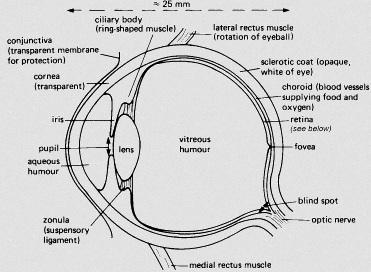
\includegraphics[width=.7\linewidth]{Eye.jpg}
\end{center}
\tiny{source: \url{http://academia.hixie.ch/bath/eye/home.html}}
\end{frame}

\begin{frame}{Eye description}
Aqueous humor : produced by the ciliary epithelium.
$\rightarrow$ drains into the Schlemm's canal.\\
Pressure produced : the intra-ocular pression (IOP).
\begin{center}
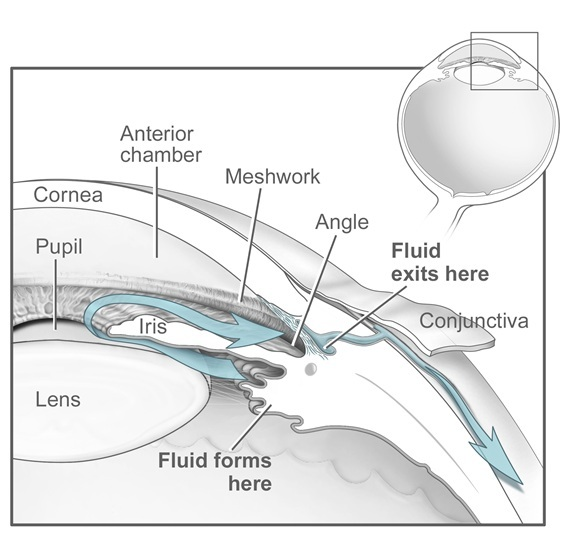
\includegraphics[width=.5\linewidth]{Humor.jpg}
\end{center}


\end{frame}

\begin{frame}{IOP}
IOP : 10 -- 22 mmHg for human (average : 16 mmHg)
\begin{itemize}
\item inflates the globe of the eye
\item measure (tonometry) takes into account the thickness 
\end{itemize}
%
%
%Note that its value can be measured by tonometry by taking into account the thickness of the cornea. A fine jet of air is directed toward the cornea.
\begin{center}
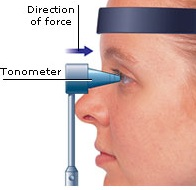
\includegraphics[scale=.6]{Tonometry.jpg}\\
\tiny{source: \url{http://www.aviva.co.uk/health-insurance/home-of-health/medical-centre/medical-encyclopedia/entry/test-tonometry/}}
\end{center}
\only<2>{\begin{center}
\ALERT{High IOP $\Rightarrow$ major risk for \textit{glaucoma}.} 
\end{center}}
\end{frame}

\begin{frame}{Glaucoma}
%The glaucoma, also called the silent thief of sight, is known as the second leading cause of blindness worldwide (1 in 40 adults over 40 years old).
%\newline
%\\
\begin{itemize}
\item Second leading cause of blindness worldwide (1 in 40 adults over 40 years old)\footnote{\textit{Relative roles of risk factors in the evaluation of a glaucoma suspect : clinical perspective and mthematical modelling},Geffen, Guidoboni, Harris \textit{et al}}
\end{itemize}
% Until now, the major risk for glaucoma is the elevated IOP but it is neither required nor enough to actually contract the disease:\\
Elevated IOP : major risk for glaucoma, but : 
\begin{itemize}
\item a patient with an elevated IOP may never contract glaucoma. 
\item a patient could have a glaucoma even though his IOP is low
\end{itemize}
\begin{center}
\alert{ 25 \% of IOP-treated patient progress to blindness}

\end{center}

\end{frame}

\begin{frame}{Glaucoma}
Group of ocular disorders with multi-factorial etiology united by a clinically characteristic optic neuropathy accompanied by a vision loss.
%\newline
%\\
There are two kinds of diagnostics: \\
\begin{itemize}
\item<2-> a morphological damage
\item<3->a physiological damage (decrease of the visual field)
\end{itemize}
\only<2>{
\begin{center}
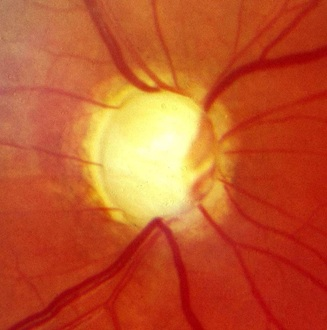
\includegraphics[scale=.5]{Morphological.jpg}\\
\tiny{Glaucomateous optic nervehead demonstrating increased cup to disc ratio}
\end{center}
The glaucoma damage the optical nerve head, where the optical nerve and blood vessels enter the retina.}
\only<3>{

\begin{center}
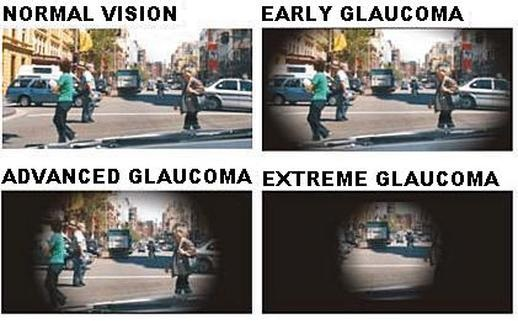
\includegraphics[scale=.5]{Glaucoma.jpg}\\
\tiny{source: \url{http://www.swisscompleteeyecare.com/uploads/3/6/3/8/3638142/8901258.jpg?520}}

\end{center}}
\only<4>{
\begin{center}
\ALERT{
However, the IOP remains the only parameter we can act on, either by surgery or with medications.
}\end{center}}
\end{frame}

\begin{frame}{Treatment}

The medications have two effects :
%: either decrease the secretion of aqueous humor or increase the elimination of it. It is also possible to combine several treatments in order to decrease even more the IOP.
\newline
\\
\begin{tabular}{|c|c|}
\hline
Decrease the secretion of aqueous humor & Increase the elimination of aqueous humor\\
\hline
beta-adrenergic receptor antagonists & Prostaglandin analogs \\
Alpha2-adrenergic agonists & Miotic agents \\
alpha agonists &  \\
Carbonic anhydrase inhibitors &  \\
\hline
\end{tabular}
\newline
\newline
It is also possible to combine several treatments in order to decrease even more the IOP.
Besides, drugs could work better on patients depending on their age, gender, ethnic group or other diseases like diabetes, hypertension...

\end{frame}

\section{Mathematical Model}

\begin{frame}{Model of intraocular fluids dynamics}
\begin{block}{}
\[
\frac{\dd U}{\dd t}=F_{h}-F_{e}
\]
\end{block}

\small{$U$: Total aqueous humor\\
$F_h$: Fluid inflow in posterior chamber\\
$F_e$: net inflow via trabecular path}
\newline
%\\
\[
F_{h}= L_p \big[ (p_a-p)-\sigma_{p} \Delta\pi_{p}-\sigma_{s} \Delta\pi_{s}\big]
\]


\small{
$L_p$: permeability of the equivalent membrane\\
$p_a$: pressure in the ciliary body capillaries\\
$p$: IOP \\
$\sigma_p$: reflection coefficient (proteins)\\
$\sigma_s$: reflection coefficient (low molecular components)\\
$\Delta \pi_p $: osmotic pressure diff. accross membrane (proteins)\\
$\Delta \pi_s $: osmotic pressure diff. across membrane (low molecular component)}

\end{frame}
\begin{frame}
\[
\Delta\pi_{s}= \rho(C_1-C_{2}) 
\]
\small{$\rho$: universal gas constant $\times$  absolute temperature\\
$C_1$: total molar concentration of low-molecular components (blood)\\
$C_2$: total molar concentration of low-molecular components (intra-ocular fluid near ciliary body surface) }
\newline
\\
\begin{block}{}
\[
 \alpha \frac{dp}{dt}=F_{h}-\frac{p-p_e}{R}
 \]
\[
 V^{\ast} \frac{dC_{2}}{dt}= Q_s-Q_e=\xi_s(C_1-C_{2})+F_h (1-\sigma_s) \bar{C}+J-F_h C_2
 \]
\end{block}
\small{
$V^\star$: volume of intraocular fluid between the folds of the ciliary body\\
$\xi_s$: average permeability of membrane for low-molecular species\\
$\overline{C}$=$\displaystyle{\frac{C_1+C_2}{2}}$\\
$J$: Influx due to active transport
$p_e$: pressure in the episcleral veins\\
$R$: output hydraulic resistance\\
$\alpha$: volume compliance of the eye shell (varies significantly)}

\end{frame}

\begin{frame}{Assumptions}

\end{frame}

\begin{frame}{Data}

\end{frame}

\section{Numerical Results}

\begin{frame}{Recovering some values}
%\pgfplotsset{
%  compat=newest,
%  xlabel near ticks,
%  ylabel near ticks
%}
\end{frame}

\begin{frame}{Summary}
-3 equations
\end{frame}




% \begin{frame}{test}
% 	Main text still in Gill Sans
% 	$$\frac{f}{f^4}$$
% 	
% 	But math is now different
% 	\Large
% 	$$\frac{f^2}{f^4}$$
% \end{frame}


\end{document}
